\documentclass[12pt]{article}
\usepackage[utf8]{inputenc}
\usepackage{graphicx} 
\usepackage{wrapfig}
\usepackage[dvipsnames]{xcolor}
\usepackage{moreverb}
\usepackage{ragged2e}
\renewcommand\refname{Referencias}
\title{Elementos de la programación Python 1.}
\author{\textcolor{JungleGreen}{Olga María Fimbres Morales}}
\date{17 de Enero 2016}
\begin{document}
\begin{titlepage}

\begin{center}
\begin{large}
Universidad del Estado de Sonora\\
\end{large}
\vspace*{0.15in}
División de Ciencias Exactas y Naturales.\\
\vspace*{0.15in}
Licenciatura en Física. \\
\vspace*{0.6in}
\begin{large}
Física Computacional 1\\
\end{large}
\vspace*{0.2in}
\begin{Large}
\textbf{{\textcolor{Red}{Iniciándose en Computo Simbólico con Maxima.}}} \\
\end{Large}

%\begin{Large}
%\textbf{{\textcolor{Red}{Péndulo.}}} \\
%end{Large}
%\vspace*{-1in}

\rule{80mm}{0.1mm}\\
\vspace*{0.1in}
\begin{large}
{\textcolor{JungleGreen}{Olga María Fimbres Morales}}\\
12 de Abril de 2016\\
\end{large}
\end{center}
\end{titlepage}

\pagebreak
\section*{Introducción.}
  A lo largo de este curso hemos podido observar como una herramienta computacional puede ayudarnos a resolver problemas que de otro modo serian sumamente complicados de resolver sin su ayuda.\\
  
  Esta vez, analizaremos la herramienta conocida como $Maxima$, que nos servirá en los momentos donde sea necesario manipular una expresión matemática; dicha herramienta cuenta con múltiples funciones y complementos que nos permiten obtener un mejor entendimiento del proceso que se lleva a cabo.\\
  
  A lo largo de esta actividad evidenciaremos un poco sobre la manera en que esta herramienta funciona y la forma en que lleva a cabo las manipulaciones correspondientes de las diferentes expresiones que son introducidas. Este reporte busca ser una corto manual para aquellos que comienzan a utilizar Maxima como herramienta de ayuda en sus actividades.
 
\section*{\textcolor{Red}{Maxima.}}
"Maxima es un sistema para la manipulación de expresiones simbólicas y numéricas". Surge de $Macsyma$, un sistema de álgebra computacional desarrollado a finales dde 1960 en el Instituto Teconológico de Massachusetts (MIT).\\
\begin{wrapfigure}{r}{6cm}
	\begin{center}
      
\includegraphics[width=5.0cm]{Maximalogo.png}
    \end{center}
\end{wrapfigure}

 Posee diferentes herramientas como la diferenciación, integración, expansión de series de Taylor, ecuaciones diferenciales, sistemas de ecuaciones lineales, vectores, matrices, entre muchas otras.\\

 Permite obtener resultados con una alta precisión gracias a que utiliza fracciones exactas, números enteros de precisión arbitraria y números de coma flotante con una variación variables. Además de esto, cuenta con un graficador que permite obtener imágenes en 2 y 3 dimensiones.\\

 La forma en que trabaja es con lenguaje Lisp, y a pesar que funciones en modo consola es posible también utilizar interfaces gráficas como $xMaxima$ y $wxMaxima$, siendo para algunos usuarios mas cómodo y sencillo utilizarlo de esta última manera.
\pagebreak
\section*{\textcolor{LimeGreen}{Problema.}}
 Llevar a cabo esta actividad consistió en realizar una serie de ejemplos correspondientes a tema de cálculo vectorial utilizando la herramienta Maxima. Cada uno de esos ejemplos seran abordados desde el punto de vista que nos interesa, es decir, la explicación de como funciones nuestra herramienta a estudiar, es por ello que no debe esperarse una larga explicación sobre cada tema, si no una breve introducción seguida del funcionamiento de Maxima.\\

 El desarrollo que se siguió en la actividad fue la de leer el manual que se nos proporcionó y apoyándonos en él se fue explorando la forma en que realiza las operaciones, además de los diversos comandos que pueden resultar comunmente utilizados para nuestra área de estudio.\\

 Cada una de los ejemplos que se llevaron a cabo fueron tomados inicialmente íntegramente como los dice el manual, mas una vez que se comprendió la forma en que estas funcionaban se procedió a modificarlas a gusto del usuario. Por lo que las funciones que se utilizaron no representan nada en específico.\\

 Se presentan además de las instrucciones utilizadas los resultados arrojados por Maxima para que de esta forma el lector pueda apreciar la forma en que esta herramienta trabaja y la manera en que te muestra los pasos utilizados.\\









\pagebreak

\section*{\textcolor{RoyalBlue}{Resultados}}
\subsection*{Geometría tridimensional.}
\subsubsection*{Vectores y Álgebra lineal.}
 Si alguna vez se ha utilizado Maple, se recordara la forma en que era necesario introducir los vectores ya que esta es la misma  manera en que debemos especificar los vectores para que Maxima los reconozca como tal; una vez que esto se ha hecho bien y a cada vector le hemos dado una etiqueta para identificarlos podremos realizar con ellos todas las operaciones que normalmente se realizan con los vectores, dígase multiplicación por un escalar, suma o resta entre ellos, producto cruz ($\sim$) y producto punto (.).\\
 \begin{verbatim}
 a: [18,86,102];
 b: [90,2,8];
 (5*a)/2;
 a + b;
 a . b;
 express(%);
 tex(sqrt(a . a));
 tex(sqrt(b . b));
 tex((a . b)/(a . a) * a);

 (%o103) [18,86,102]
 (%o104) [90,2,8]
 (%o105) [45,215,255]
 (%o106) [108,88,110]
 (%o107) 2608
 (%o108) express(2608)
 $2\,\sqrt{4531}$
 (%o109) false
 $$2\,\sqrt{2042}$$
 (%o110) false
 $$\left[ {{11736}\over{4531}} , {{56072}\over{4531}} , {{66504}\over{
 4531}} \right] $$
 (%o111) false
 \end{verbatim}

\subsubsection*{Lineas, planos y superficies.}
 Maxima cuenta con una herramienta de graficación integrada que nos permite realizar diferentes diagramas de funciones lineales, gráficas en 2 y en 3 dimensiones que además estas últimas resultan ser interactivas ya que es posible mover las gráficas para obtener una mejor visión y apreciación de lo que realizamos.\\

 Este ejemplo es el de una superficie tridimensional, donde inicialmente es necesario especificar la figura con la que se estará trabajando, a continuación cargar la herramienta necesaria y por último dar la instrucción que realize la gráfica donde además se especifican los valores de los ejes y los colores que tendrá la misma.\\

\begin{verbatim}
 plane1: 3*x + 4*y + 5*z = 0;
 (%o1) 5*z+4*y+3*x=0

 load(draw);
 (%o3) "/usr/share/maxima/5.32.1/share/draw/draw.lisp"

 draw3d(enhanced3d = true, implicit(plane1, x, -4,4, y, -4,4, z, -6,6),
 palette=[20,-13,0]);
 (%o4) [gr3d(implicit)]
 \end{verbatim}

 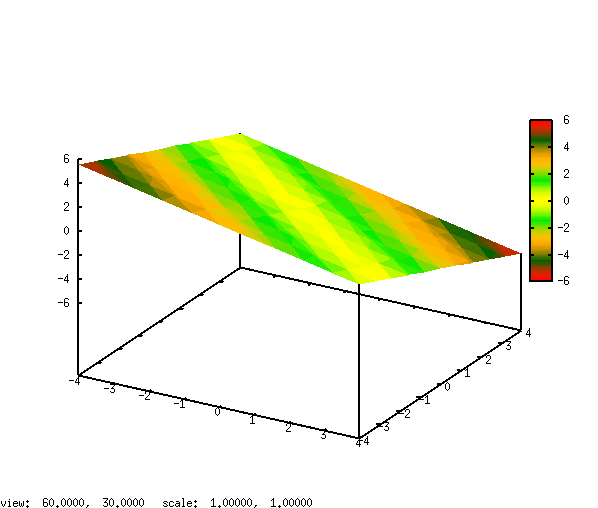
\includegraphics[scale=0.4]{actividad80.png}

 \begin{verbatim}
 hyperboloid: x^2 + y^2 - z^2 = 1;
 (%o5) −z^2+y^2+x^2=1

 draw3d(enhanced3d = true, implicit(hyperboloid, x, -5,5, y, -2.5,2.5, z, -4,4),
 palette=[10,23,-1]);
 (%o6) [gr3d(implicit)]
 \end{verbatim}

 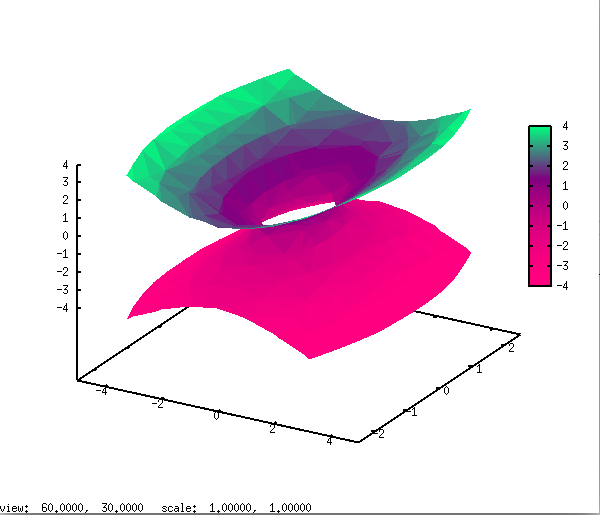
\includegraphics[scale=0.4]{actividad8.png}

\subsubsection*{Funciones vectoriales evaluadas.}

 En esta herramienta también es posible utilizar funciones definidas, como las trigonométricas por ejemplo, que podemos utilizar para definir funciones vectoriales.\\

 Además de esto es posible evaluar dichas funciones y obtener un valor específico si es que asi lo queremos.

 \begin{verbatim}
 r(t) := [t, cos(t), sin(t)];
 r(1);
 float(%);
 load(draw);
 draw3d(parametric(cos(t), -cos(t), sin(t), t, 8, 12));
 limit(r(t), t, 2);
 float(%);
 limit(r(t), t, 2, plus);
 limit(r(t), t, 3, minus);
 diff(r(t), t);
 define(rp(t), diff(r(t), t));
 float(rp(1));
 load(eigen);
 uvect(rp(t));
 trigsimp(%);
 define(T(t), %);
 define(Tp(t), diff(T(t), t));
 uvect(Tp(t));
 trigsimp(%);
 define(N(t), %);
 load(vect);
 \end{verbatim}
 Los resultados que arrojan son los siguientes de manera ordenada:
 \begin{verbatim}
 (%o22) r(t):=[t,cos(t),sin(t)]
 (%o23) [1,cos(1),sin(1)]
 (%o24) [1.0,0.54030230586813,0.84147098480789]
 (%o25) "/usr/share/maxima/5.32.1/share/draw/draw.lisp"
 (%o26) [gr3d(parametric)]
 (%o27) [2,cos(2),sin(2)]
 (%o28) [2.0,−0.41614683654714,0.90929742682568]
 (%o29) [2,cos(2),sin(2)]
 (%o30) [3,cos(3),sin(3)]
 (%o31) [1,−sin(t),cos(t)]
 (%o32) rp(t):=[1,−sin(t),cos(t)]
 (%o33) [1.0,−0.84147098480789,0.54030230586813]
 (%o34) "/usr/share/maxima/5.32.1/share/matrix/eigen.mac"
 (%o35)
 \end{verbatim}
 $$\left[ {{1}\over{\sqrt{\sin ^2t+\cos ^2t+1}}} , -{{\sin t}\over{
 \sqrt{\sin ^2t+\cos ^2t+1}}} , {{\cos t}\over{\sqrt{\sin ^2t+\cos ^2
 t+1}}} \right] $$
 \begin{verbatim}
 (%o36) 
 \end{verbatim}
 $$\left[ {{1}\over{\sqrt{2}}} , -{{\sin t}\over{\sqrt{2}}} , {{\cos t
 }\over{\sqrt{2}}} \right] $$
 \begin{verbatim}
 (%o37) T(t):=[1/sqrt(2),−sin(t)/sqrt(2),cos(t)/sqrt(2)]
(%o38) Tp(t):=[0,−cos(t)/sqrt(2),−sin(t)/sqrt(2)]
(%o39) [0,−cos(t)/sqrt(sin(t)^2+cos(t)^2),−sin(t)/sqrt(sin(t)^2+cos(t)^2)]
(%o40) [0,−cos(t),−sin(t)]
(%o41) N(t):=[0,−cos(t),−sin(t)]
tellsimpafter: circular rule attempted.
 -- an error. To debug this try: debugmode(true);
\end{verbatim}
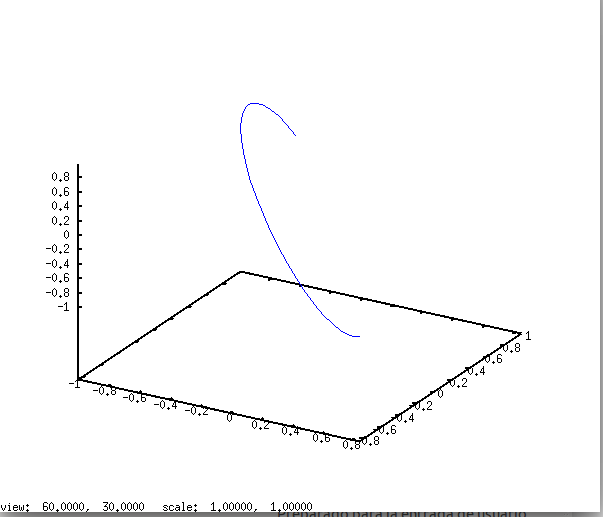
\includegraphics[scale=0.4]{actividad81.png}

Como podemos observar, inicialmente especificamos la función con la estaríamos trabajando y la evaluamos en un valor deseado, este será mostrado de diferentes maneras, ya que puede ser presentado como las funciones evaluadas o bien como los valores reales de estas.\\

Comenzamos además a utilizar la herramienta $diff$, que como podemos ver es referente a la derivada de la función con la que estamos trabajando, mostrando así nuevamente el vector pero derivado con respecto a la variable utilizada. Igualmente, este nuevo vector puede ser evaluado y mostrado de ambas maneras anteriormente mencionadas.\\

A continuación podemos observar la instrucción $uvect$, que nos permite normalizar un vector y convertirlo en uno unitario, es decir, que su magnitud será 1. Permitiéndonos aplicar identidades trigonométricas por medio de $trigsimp$ y de esta forma simplificar la forma en que se da el vector.

\subsubsection*{Longitud de arco y curvatura.}
\begin{verbatim}
r(t) := [t, cos(t)+2, sin(t^2)];
rp(t) := [1, -5*sin(t), cos(t)-3];
Tp(t) := [0, -8*cos(t^2), sin(t)+1]/sqrt(2);
sqrt(Tp(t) . Tp(t))/sqrt(rp(t) . rp(t));
trigsimp(%);
definne(kappa(t), %);
integrate(r(t),t);
\end{verbatim}
Esto nos arroja los siguientes resultados:
\begin{verbatim}
(%o12) r(t):=[t,cos(t)+2,sin(t^2)]
(%o13) rp(t):=[1,(−5)*sin(t),cos(t)−3]
(%o28) Tp(t):=([0,(−8)*cos(t^2),sin(t)+1])/sqrt(2)
(%o31) sqrt(32*cos(t^2)^2+(sin(t)+1)^2/2)/sqrt(25*sin(t)^2+(cos(t)−3)^2+1)
(%o32) sqrt(64*cos(t^2)^2+sin(t)^2+2*sin(t)+1)/(sqrt(2)*sqrt(−24*cos(t)^2−6*cos(t)+35))
(%o17) definne(kappa(t),sqrt(64*cos(t^2)^2+sin(t)^2+2*sin(t)+1)/(sqrt(2)*sqrt(−24*cos(t)^2−6*cos(t)+35)))
(%o18) [t^2/2,sin(t)+2*t,(sqrt(%pi)*((sqrt(2)*%i+sqrt(2))*erf(((sqrt(2)*%i+sqrt(2))*t)/2)+(sqrt(2)*%i−sqrt(2))*erf(((sqrt(2)*%i−sqrt(2))*t)/2)))/8]
\end{verbatim}

De esto podemos observar como también es posible realizar integraciones utilizando Maxima, siendo mucha mas cómoda la salida para wxMaxima que la que se nos presenta, dentro del mismo programa, para salida a Latex.\\

Podemos analizar las mismas operaciones de una forma distinta:
\begin{verbatim}
g(t):=[2*t^4,2*sin(t),cos(t)-5];
define(gp(t),diff(g(t),t));
integrate(trigsimp(sqrt(gp(t).gp(t))),t,0,2*%pi);
romberg(sqrt(gp(t).gp(t)),t,0,2*%pi);
\end{verbatim}
Obteniendo como resultado:
\begin{verbatim}
(%o23) g(t):=[2*t^4,2*sin(t),cos(t)−5]
(%o24) gp(t):=[8*t^3,2*cos(t),−sin(t)]
(%o25) integrate(sqrt(3*cos(t)^2+64*t^6+1),t,0,2*%pi)
(%o26) 3118.2238495674
\end{verbatim} 

Como podemos apreciar esta vez, aunque utilizamos las mismas instrucciones que en el ejemplo anterior resulta mas cómodo y compacto si combinamos las instrucciones y calculamos una misma expresión mientras que le aplicamos mas de una herramienta.

\subsection*{Funciones de varias variables.}
\subsubsection*{Derivadas parciales.}

\begin{verbatim}
diff(f(x,y),x);
diff(diff(f(x,y),x),x);
diff(diff(f(x,y),x),y);
\end{verbatim}

$${{d}\over{d\,x}}\,f\left(x , y\right)$$
$${{d^2}\over{d\,x^2}}\,f\left(x , y\right)$$
$${{d^2}\over{d\,x\,d\,y}}\,f\left(x , y\right)$$

Podemos ver que para realizar derivadas parciales utilizamos la instrucción $diff$, pero a diferencia de como la utilizamos anteriormente, esta vez después de especificar la función a la que nos referimos debemos de especificar la variables respecto a la cual deseamos realizar la derivación. Además de esto, si desea realizarse mas de una vez basta con agregar nuevamente la instrucción junto con la función ya derivada y la variable que será considerada.

\begin{verbatim}
G:(x^6 +2) *y^-2;
diff(G,x,1,y,2,x,3);
diff(G,x,1);
diff(G,y,2);
\end{verbatim}

$${{x^6+2}\over{y^2}}$$
$${{2160\,x^2}\over{y^4}}$$
$${{6\,x^5}\over{y^2}}$$
$${{6\,\left(x^6+2\right)}\over{y^4}}$$

Con este nuevo ejemplo podemos observar una nueva forma de realizar derivadas parciales múltiples de una forma más compacta, ya que basta con especificar la función a derivas, la variables respecto a la cual se hará y el número de veces que se desea realizar esta operación; lo que resulta más cómodo es el hecho de que dentro de una misma instrucción es posible señalar diversas derivadas parciales y el orden en que desea sean realizadas.

\subsubsection*{Aproximación lineal y diferenciales.}

Por medio de la herramienta $taylor$ podemos obtener un desarrollo en series de Taylor de la función que especifiquemos, siendo esto sumamente útil cuando trabajamos con series muy grandes que resultan mas sencillas analizar si se tienen de una manera simplificada o simplemente manejar una aproximación a la expresión de forma que las operaciones que debamos de realizar sean mucho mas sencillas.
\begin{verbatim}
f(x,y):= exp(x^2) * sin(y^3)+8;
taylor(f(x,y),[x,y],[1,2],1);
diff(f(x,y));
\end{verbatim}

\begin{verbatim}
f(x,y):=exp(x^2)*sin(y^3)+8;
\end{verbatim}
$$8+\sin 8\,e+\left(2\,\sin 8\,e\,\left(x-1\right)+12\,\cos 8\,e\,
 \left(y-2\right)\right)+\cdots $$
 $$3\,e^{x^2}\,y^2\,\cos y^3\,{\it del}\left(y\right)+2\,x\,e^{x^2}\,
  \sin y^3\,{\it del}\left(x\right)$$
  
  \subsubsection*{Regla de la cadena y diferenciaci\'on implicita.}
  
  Como sabemos la regla de la cadena se aplica cuando una sola expresión depende de dos diferentes variables o bien una sola expresión encierra distintas operaciones que se aplican sobre la variables respecto a la cual nos encontramos derivando.\\
  
  Maxima nos permite realizar este proceso de una manera sencilla, tal como se muestra en el siguiente ejemplo:
  \begin{verbatim}
  f(x,y) := exp(x^4) * sin(y)+8;
  [x,y] : [s^2 * t, s * t^2];
  diff(f(x,y),s);
  diff(f(x,y), t);
  diff(f(x,y),x);
  diff(f(u,v),u);
  \end{verbatim}
  
  \begin{verbatim}
  f(x,y):=exp(x^4)*sin(y)+8;
  \end{verbatim}
  $$\left[ s^2\,t , s\,t^2 \right] $$
  $$8\,s^7\,t^4\,e^{s^8\,t^4}\,\sin \left(s\,t^2\right)+t^2\,e^{s^8\,t^
   4}\,\cos \left(s\,t^2\right)$$
   $$4\,s^8\,t^3\,e^{s^8\,t^4}\,\sin \left(s\,t^2\right)+2\,s\,t\,e^{s^8
    \,t^4}\,\cos \left(s\,t^2\right)$$
    $diff: second argument must be a variable; found s^2*t$
    $$4\,u^3\,e^{u^4}\,\sin v$$
    
    Podemos observar que al inicio se especificó la función con la que se trabajaría, después de esto se realizo una nueva definición de las variables $x$ y $y$ por medio de un nuevo vector, logrando así una composición con ambas expresiones que mas tarde se pediría derivar parcialmente respecto a diversas variables; permitiéndonos observas que además de respetar esto se realiza la derivación correctamente utilizando la regla de la cadena correspondiente a cada caso.\\
    
    Mostrando nuevamente como esta herramienta resulta sumamente conveniente cuando lo que necesitamos es realizar este tipo de operaciones de manera rápida para poder concentrarnos en otras operaciones o problemas más complejos.
  
  \subsubsection*{Derivadas direccionales y gradiente.}
  
  Otro concepto muy utilizado en un cálculo más avanzado es el de gradiente, el cual podemos definir como el vector en el cual una función tendrá un crecimiento más rápido; sabemos que para calcular el gradiente de una función es necesario realizar una derivada parcial con cada una de la variables a la misma función y este resultado nos indicará el gradiente de la función. La herramienta de Maxima nos permite realizarlo de una forma sumamente sencilla que se resume a utilizar una simple instrucción:
  \begin{verbatim}
  f(x,y) := exp(x^2)*sin(y^3)-5;
  load(vect);
  scalefactors([x,y]);
  gdf: grad(f(x,y));
  ev(express(gdf), diff);
  define(gdf(x,y),%);
  v:[3,4];
  (gdf(1,2).v)/sqrt(v.v);
  ev(%,diff);
  float(%);
  sqrt(gdf(1,2).gdf(1,2));
  float(ev(%,diff));
  \end{verbatim}
  
  Obtenemos cono resultado lo siguiente de una forma ordenada y correspondiente a cada instrucción que introducimos en Maxima, como podemos observar, solo basta con especificar la función a trabajar y utilizar la instrucción correspondiente al gradiente. Que una vez utilizado es posible evaluar y realizar operaciones con el.
  \begin{verbatim}
  f(x,y):=exp(x^2)*sin(y^3)-5;
  (%o2) "/usr/share/maxima/5.32.1/share/vector/vect.mac"
  (%o3) done
  (%o28)
  \end{verbatim}
  $${\it grad}\left(e^{x^2}\,\sin y^3-5\right)$$
  $$\left[ 2\,x\,e^{x^2}\,\sin y^3 , 3\,e^{x^2}\,y^2\,\cos y^3 \right] $$
  \begin{verbatim}
  gdf(x,y):=text(gdf(x,y):=text(gdf(x,y):=false));
  (%o7) [3,4]
  (%o36)
  \end{verbatim}
  $${{6\,e\,\sin 8+48\,e\,\cos 8}\over{5}}$$
  $${{6\,e\,\sin 8+48\,e\,\cos 8}\over{5}}$$
  \begin{verbatim}
  (%o10) −0.56967148788552
  (%o39)
  \end{verbatim}
  $$\sqrt{4\,e^2\,\sin ^28+144\,e^2\,\cos ^28}$$
  \begin{verbatim}
  (%o12) 7.173296150035195
  \end{verbatim}
  
  \subsubsection*{Optimización.}
  
  Para algunos problemas es necesario saber en que puntos una función es mínima o máxima, sabemos que una forma de realizar este análisis es por medio del criterio de las derivadas, donde los puntos importantes es donde estas toman un valor de 0, para después analizar si estos puntos corresponden a mínimos o máximos.
  \begin{verbatim}
  f(x,y) := 2*x^3 + 3*y^4 - 5*x^2*y;
  load(draw);
  draw3d(enhanced3d=true, explicit(f(x,y),x,-3,3,y,-2,2),palette=[5,0,20]);
  draw3d(explicit(f(x,y),x,-3,3,y,-2,2),contour=map);
  fx:diff(f(x,y),x);
  fy:diff(f(x,y),y);
  solve([fx,fy],[x,y]);
  H:hessian(f(x,y),[x,y]);
  determinant(H);
  subst([x=-1,y=-1],diff(fx,x));
  subst([x=-1,y=-1],determinant(H));
  f(-1,-1);
  \end{verbatim}
  
Los resultados que nos muestra de forma ordenada son los siguientes, donde podemos observar que se realizo la derivada parcial de la función, de la forma vista anteriormente para esta vez encontrar los puntos donde estas arrojan el valor de 0, es decir, donde la función puede ser un máximo:
  
  \begin{verbatim}
  f(x,y):=2*x^3+3*y^4+(-5)*x^2*y;
  (%o15) "/usr/share/maxima/5.32.1/share/draw/draw.lisp"
  (%o17) [gr3d(explicit)]
  (%o18) [gr3d(explicit)]
  (%o28)
  \end{verbatim}
  $$6\,x^2-10\,x\,y$$
  \begin{verbatim}
  (%o29)
  \end{verbatim}
  $$12\,y^3-5\,x^2$$
  \begin{verbatim}
  (%o30)
  \end{verbatim}
  $$\left[ \left[ x=0 , y=0 \right]  , \left[ x={{625}\over{324}} , y=
   {{125}\over{108}} \right]  \right] $$
   \begin{verbatim}
   (%o31)
   \end{verbatim}
   $$\pmatrix{12\,x-10\,y&-10\,x\cr -10\,x&36\,y^2\cr }$$
   \begin{verbatim}
   (%o32)
   \end{verbatim}
   $$36\,\left(12\,x-10\,y\right)\,y^2-100\,x^2$$
   \begin{verbatim}
   (%o24) −2
   (%o25) −172
   (%o26) 6
   \end{verbatim}
   
   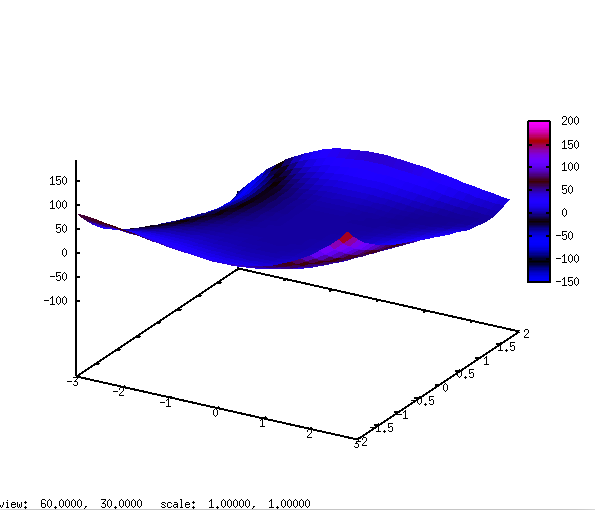
\includegraphics[scale=0.4]{actividad82.png}
   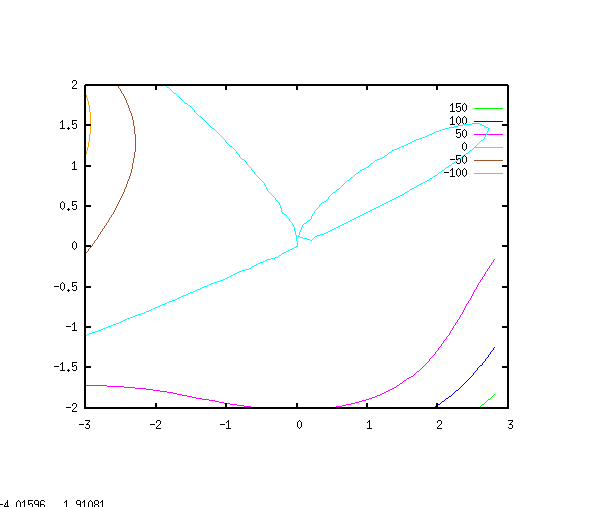
\includegraphics[scale=0.4]{actividad83.png}
   \pagebreak
   \subsubsection*{Multiplicadores de Lagrange.}
   
   Los multiplicadores de Lagrange se utilizan para encontrar los máximos y mínimos de una función que se encuentra sujeta a restricciones; reduciendo el problema restringido a uno sin restricciones con un mayor número de variables cuyas ecuaciones resultan mas sencillas de resolver.\\
   
   El siguiente ejemplo requiere que le demos una función con la cual trabajar y a partir de la cual obtendremos otras tres ecuaciones las cuales resolveremos por el método de multiplicadores de Lagrange.
   
   \begin{verbatim}
   f(x,y) := 8*x^3 + y^2 - 5;
   g:x^2 + 2*y^3;
   eq1:diff(f(x,y),x)=h*diff(g,x);
   eq2: diff(f(x,y),y)=h*diff(g,y);
   eq3:g=1;
   solve([eq1,eq2,eq3],[x,y,h]);
   [f(1,0),f(-1,0),f(0,-1),f(0,1)];
   \end{verbatim}
   
   Obteniendo los siguientes resultados:
   
   \begin{verbatim}
   (%029)f(x,y):=8*x^3+y^2-5;
   (%030)
   \end{verbatim}
   $$2\,y^3+x^2$$
   \begin{verbatim}
   (%031)
   \end{verbatim}
   $$24\,x^2=2\,h\,x$$
   \begin{verbatim}
   (%o32)
   \end{verbatim}
   $$2\,y=6\,h\,y^2$$
   \begin{verbatim}
   (%o33)
   \end{verbatim}
   $$2\,y^3+x^2=1$$
   \begin{verbatim}
   (%o34) *valores de [x,y,h] en anexo
   (%o28) [3,−13,−4,−4]
   \end{verbatim}
   
   \subsection*{Integración Múltiple.}
   \subsubsection*{Integrales dobles.}
   
   Las integrales dobles las utilizamos en diversos problemas, principalmente en el calculo de áreas; Maxima permite, al igual que  las derivadas, realizar una integración sobre otra, sencillamente indicando nuevamente que se desea llevar a cabo este procedimiento, tal como se muestra en el siguiente ejemplo:
   \begin{verbatim}
   f(x,y):=5*x^8 -3*x^2*y;
   integrate(integrate(f(x,y),y),x);
   integrate(integrate(f(x,y),y,x^1/2,2-x),x,0,1);
   \end{verbatim}
   Resultados:
   \begin{verbatim}
   (%o4)f(x,y):=5*x^8-3*x^2*y;
   (%o5)
   \end{verbatim}
   $${{5\,x^9\,y}\over{9}}-{{x^3\,y^2}\over{2}}$$
  \begin{verbatim}
  (%o6)
  \end{verbatim}
  $$-{{131}\over{360}}$$
  
  \subsubsection*{Integración en coordenadas polares.}
  
  En algunos escenarios es necesario realizar un cambio de coordenadas y que de este modo la integración resulte mucho más sencilla de realizar. Maxima nos permite realizar este cambio de coordenadas sin mayor complicación ya que el procedimiento es de la manera obvia, es decir realizando la sustitución que estamos acostumbrados a utilizar.
  
  \begin{verbatim}
  f(x,y):=3*x^4+3*y^4;
  [x,y]:[r*cos(theta),r*sin(theta)];
  integrate(integrate(f(x,y)*r,r,0,2*cos(theta)),theta,-%pi/2,%pi/2);
  \end{verbatim}
  
  Como podemos ver a continuación en los resultados el proceso resulta rápido y resumido, siendo capaces de integrar bajo los límites que necesitemos simplemente especificándolos dento de la instrucción de integración.
  
  \begin{verbatim}
  (%010) f(x,y):=3*x^4+3*y^4;
  (%011)
  \end{verbatim}
  $$\left[ r\,\cos \vartheta , r\,\sin \vartheta \right] $$
  \begin{verbatim}
  (%012)
  \end{verbatim}
  $${{33\,\pi}\over{4}}$$
  
  \subsubsection*{Integrales triples.}
  
  De una manera similar con las integrales dobles, las integrales triples utilizadas en diversos contextos del cálculo como por ejemplo para encontrar densidades o bien volúmenes.\\
  
  Tal como podemos ver en el ejemplo basta con realizar lo mismo que sabemos podemos hacer con las derivadas, es decir, realizar la misma instrucción repetidas veces, especificando en cada caso la variable respecto a la cual se integrará y los limites bajo los cuales se evaluará.
  \begin{verbatim}
  integrate(integrate(integrate(2*x^5*y^3*z^2,z,0,2*x^3+2*y),y,0,-3*x^3),x,0,2);
  (%02)
  \end{verbatim}
  $$-{{68182605824}\over{35}}$$
  
  \subsubsection*{Integrales en coordenadas cilíndricas y esféricas.}
  
  De manera similar a como Maxima maneja las coordenadas polares, podemos realizar una integración en otros sistemas de coordenadas, como lo son las coordenadas cilíndricas y las esféricas; en ambos casos realizando la sustitución del modo en que estamos acostumbrados. Y ya que en ambos casos las utilizamos para volúmenes realizamos una triple integración especificando la variable a integrar y los límites bajo los que se realizará.
  
  \begin{verbatim}
  /*Integrales en coordenadas cilindricas*/
  f(x,y,z):=6*x^3*y^2*z;
  [x,y,z]:[r*cos(theta),r*sin(theta),z];
  integrate(integrate(integrate(f(x,y,z)*r,z,-2,3),r,0,4),theta,-%pi/2,%pi);
  \end{verbatim}
  
  Resultados obtenidos de la integración en coordenadas cilíndricas:
  
  \begin{verbatim}
  (%011)f(x,y,z):=6*x^3*y^2*z;
  (%012)
  \end{verbatim}
  $$\left[ r\,\cos \vartheta , r\,\sin \vartheta , \rho\,\cos \vartheta
    \right] $$
  \begin{verbatim}
  (%013)
  \end{verbatim}
  $${{32768}\over{7}}$$
  
 
  
  \begin{verbatim}
  /*Integrales en coordenadas esféricas*/
  kill(f,x,y,z);
  f(x,y,z) := 2*x^3*z;
  [x,y,z] : [rho*sin(phi)*cos(theta), rho*sin(phi)*sin(theta), rho*cos(theta)];
  integrate(integrate(integrate(f(x,y,z)*rho^2*sin(phi),rho,0,1),theta,0,%pi),
  phi,0,%pi/2);
  \end{verbatim}
  
  Resultados obtenidos de la integración en coordenadas esféricas:
  \begin{verbatim}
  (%o5) done
  (%06) f(x,y,z):=2*x^3*z;
  (%08)
  \end{verbatim}
  $$\left[ \sin \varphi\,\rho\,\cos \vartheta , \sin \varphi\,\rho\,
   \sin \vartheta , \rho\,\cos \vartheta \right] $$
  \begin{verbatim}
  (%o9)
  \end{verbatim} 
  $${{9\,\pi^2}\over{448}}$$
  \pagebreak
  \subsubsection*{Cambio de variables.}
  
  Para terminar con los tipos de integraciones, hablaremos del cambio de variable por medio de la transformación más genera; además de esto, sabemos que es necesario el determinando del jacobiano de la transformación y su determinante, por lo que lo obtenemos por medio de la instrucción $jacobian$ y $determinant$ respectivamente.
  
  \begin{verbatim}
  /*Cambio de variable*/
  f(x,y):=3*x^4+y^6;
  [x,y]: [2*u^3 - v^4, 8 * u^3 * v^2];
  J:jacobian([x,y],[u,v]);
  J:determinant(J);
  integrate(integrate(f(x,y)*J,u,1,2),v,3,4);
  \end{verbatim}
  
  Resultados obtenidos:
  
  \begin{verbatim}
  (%o10)f(x,y):=3*x^4+y^6;
  (%o11)
  \end{verbatim}
  $$\left[ 2\,u^3-v^4 , 8\,u^3\,v^2 \right] $$
  \begin{verbatim}
  (%o12)
  \end{verbatim}
  $$\pmatrix{6\,u^2&-4\,v^3\cr 24\,u^2\,v^2&16\,u^3\,v\cr }$$
  \begin{verbatim}
  (%o13)
  \end{verbatim}
  $$96\,u^2\,v^5+96\,u^5\,v$$
  \begin{verbatim}
  (%o14)
  \end{verbatim}
  $${{4886568268564153324088824}\over{495}}$$
  \pagebreak
  
  \subsection*{Cálculo vectorial.}
  \subsubsection*{Campo vectorial.}
  
  Como sabemos, el campo vectorial es la representación gráfica de la distribución de de los vectores. Este puede ser en dos dimensiones, en tres o ser formado por gradientes.
  
  \begin{verbatim}
  */Campos vectoriales 2d*/
  load(draw);
  F(x,y) := [3*sin(y^4),3*x^2 + 6];
  coord: setify(makelist(k,k,-4,4));
  points2d: listify(cartesian_product(coord,coord));
  vf2d(x,y) := vector([x,y],[3*sin(y^4),3*x^2 + 6]/6);
  vect2: makelist(vf2d(k[1],k[2]),k,points2d);
  apply(draw2d,append([color=green],vect2));
  \end{verbatim}
  
  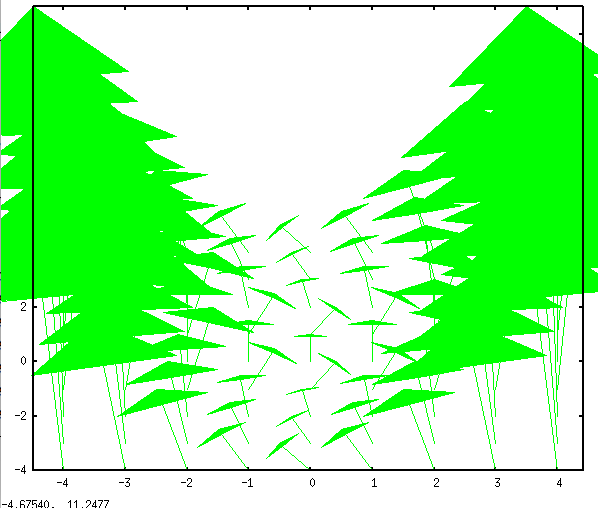
\includegraphics[scale=0.4]{actividad84.png}
   
   \begin{verbatim}
   /*campo vectorial de gradientes*/
   load(draw);
   kill (f , x , y , gdf );
   f (x , y ) := x^2 - y^2;
   scalefactors ([ x , y ]);
   gdf (x , y ) := grad ( f (x , y ));
   ev ( express ( gdf (x , y )) , diff );
   define ( gdf (x , y ) , %);
   coord : setify ( makelist (k ,k , -4 ,4));
   points2d : listify ( cartesian_product ( coord , coord ));
   vf2d (x , y ) := vector ([ x , y ] , gdf (x , y )/8);
   vect2 : makelist ( vf2d ( k [1] , k [2]) , k , points2d );
   apply ( draw2d , append ([ head_length =0.1 , color = pink ] , vect2 ));
   \end{verbatim}
   
  \begin{verbatim}
  */Campo vectorial 3d*/
  load(draw);
  coord : setify ( makelist (k ,k , -5 ,2));
  points3d : listify ( cartesian_product ( coord , coord , coord ));
  vf3d (x ,y , z ):= vector ([ x ,y , z ] ,[z+1 ,x^2 , y ]/8);
  vect3 : makelist ( vf3d ( k [1] , k [2] , k [3]) , k , points3d );
  apply ( draw3d , append ([ color = red ] , vect3 ));
  \end{verbatim}
  
  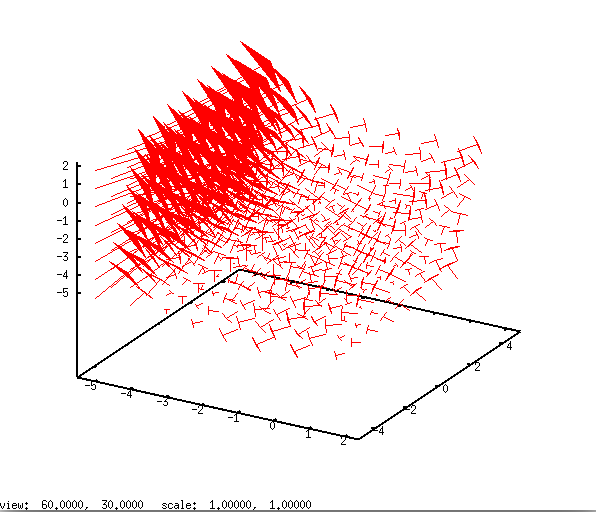
\includegraphics[scale=0.5]{actividad85.png}
\pagebreak

\subsubsection*{Integrales de línea.}

Las integrales de línea es aquella donde su función es evaluada sobre una curva; puede utilizarse para conocer el área de una curva proyectada a una superficie,para el calculo de la longitud de de la curva en el espacio, o bien para el calculo del trabajo al mover un objeto a lo largo de una trayectoria.\\

Apoyándonos en las formulas que ya conocemos podemos realizar los cálculos necesarios utilizando Maxima con la instrucción $diff$ y $romberg$ la cual realiza una integración por el método de Rombergs y nos regresa una estimación de la integral.

\begin{verbatim}
/*con respecto a la longitud de arco*/
f(x,y) := 5*x^3 + 8*y - 9;
[x,y]: [cos(t),sin(2*t)];
rp: diff([x,y],t);
romberg(f(x,y)*sqrt(rp.rp),t,0,1);
\end{verbatim}

\begin{verbatim}
(%o29) f(x,y):=5*x^3+8*y-9;
(%o30)
\end{verbatim}
$$\left[ \cos t , \sin \left(2\,t\right) \right] $$
\begin{verbatim}
(%o31)
\end{verbatim}
$$\left[ -\sin t , 2\,\cos \left(2\,t\right) \right] $$
\begin{verbatim}
(%o32) −0.67131093463861
\end{verbatim}

O bien podemos realizar una integración de línea por medio de campos vectoriales, además de desarrollar una derivada respecto al cambio de variable utilizamos también el método de Rombergs.

\begin{verbatim}
/* campos vectoriales*/
F(x,y,z) := [2*x^4*y^2, x^2*z, 6*y*z^5];
[x,y,z]: [t^5, t^3, t^2];
romberg(F(x,y,z) . diff([x,y,z], t), t, 0, 1);
\end{verbatim}

\begin{verbatim}
(%o37)F(x,y,z):=[2*x^4*y^2,x^2*z,6*y*z^5];
(%o38) 
\end{verbatim}
$$\left[ t^5 , t^3 , t^2 \right] $$
\begin{verbatim}
(%o39) 1.322580645408459
\end{verbatim}

\pagebreak
\subsubsection*{Campo vectorial conservativo.}

Un campo vectorial $F$ se dice conservativo si existe una función $f$ tal que el gradiente de dicha función sea igual a la función $F$.\\

Utilizando Maxima podemos decir si un campo es conservativo o no apoyándonos en la función $curl$, ya que si esta resulta ser $0$, diremos que el campo es conservativo.

\begin{verbatim}
F(x,y) := [x^3 - 8*y^4, 6*y^2 - 5*x^3];
load(vect);
scalefactors([x,y]);
curl(F(x,y));
express(%);
ev(%, diff);
\end{verbatim}

Este campo nos arroja los siguientes resultados:

\begin{verbatim}
F(x,y):=[x^3-8*y^4,6*y^2-5*x^3];
(%o1) false
(%o2) "/usr/share/maxima/5.32.1/share/vector/vect.mac"
(%o3) done
(%o4)
\end{verbatim}
$${\it curl}\left(\left[ x^3-8\,y^4 , 6\,y^2-5\,x^3 \right] \right)$$
\begin{verbatim}
(%o5)
\end{verbatim}
$${{d}\over{d\,x}}\,\left(6\,y^2-5\,x^3\right)-{{d}\over{d\,y}}\,
 \left(x^3-8\,y^4\right)$$
\begin{verbatim} 
(%o6) 
\end{verbatim}
$$32\,y^3-15\,x^2$$

Ya que el $curl$ no arrojó como resultado $0$, diremos que este campo no es conservativo.\\
De esta forma podemos comprobar distintos campos y conocer si son o no son conservativos

\pagebreak
\section*{\textcolor{Orange}{Conclusiones.}}

Como podemos observar, Maxima resulta una herramienta sumamente útil al momento de desarrollar diversas tareas algebraicas que de otro modo podrían llevarnos una gran cantidad de tiempo o incluso no podríamos llegar a un resultado útil.\\

La forma en que trabaja Maxima nos permite decidir si mostramos paso por paso el procedimiento o bien si deseamos únicamente conocer el resultado final, todo simplemente por la forma en que introduzcamos las instrucciones.\\

Además de esto, el hecho de que cuente con un graficador integrado permite realizar un análisis mas a fondo de algunos problemas donde las respuestas surgen de una forma visual.\\

Cuenta con diversas plataformas de trabajo, ya sea desde la terminal, con el escritorio de wxMaxima o incluso la plataforma en línea donde se incluye además una serie de etiquetas que permiten encontrar de manera rápida las instrucciones y la forma en que trabajan cada una.


 
\pagebreak
\section*{\textcolor{Purple}{Anexos}}
   $$\left[ \left[ x=1 , y=0 , h=12 \right], \left[ x=-1 , y=0 , h=-12 \right]$$
    $$\left[ x=7.450580596923828 \times 10^{-9}-
     7.450580596923828 \times 10^{-9}\,i , y=0.6873648184993\,i-
     0.39685026299204 , h=-0.36370787865724\,i-0.20998684164914 \right]$$ $$\left[ x=7.450580596923828 \times 10^{-9}\,i-
    7.450580596923828 \times 10^{-9} ,  y=0.6873648184993\,i-
    0.39685026299204 , 
    h=-0.36370787865724\,i-0.20998684164914 \right]$$ $$\left[ x=-7.450580596923828 \times 10^{-9}\,i-
    7.450580596923828 \times 10^{-9} , y=-0.6873648184993\,i-
    0.39685026299204 , h=0.36370787865724\,i-0.20998684164914 \right]$$ $$\left[ x=7.450580596923828 \times 10^{-9}\,i+
    7.450580596923828 \times 10^{-9} , y=-0.6873648184993\,i-
    0.39685026299204 , h=0.36370787865724\,i-0.20998684164914 \right]$$ $$\left[ x=-1.4901161193847656 \times 10^{-8} , y=0.79370049732915
     , h=0.41997371879106 \right]$$ 
     $$\left[ x=1.4901161193847656 \times 10^{-8} , y=0.79370049732915 , h=
    0.41997371879106 \right]$$ $$\left[ x=0.035012119579854 , y=
    0.79337606837606 , h=0.42014543495825 \right]$$ $$\left[ x=
    0.03030896972345\,i-0.017484626183968 , y=-0.68764545661009\,i-
    0.39668863262709 , h=0.3637076366814\,i-0.20981551420761 \right]$$ $$\left[ x=-0.03030896972345\,i-0.017484626183968 , y=0.68764545661009
    \,i-0.39668863262709 , h=-0.3637076366814\,i-0.20981551420761
    \right]$$ $$\left[ x=0.99997856469176 , y=0.027778373624487 , h=
    11.9997427321842 \right]$$ $$\left[ x=-1.000021432092415 , y=-
    0.027777182416357 , h=-12.00025720164609 \right]  \right] $$

\pagebreak
\begin{thebibliography}{X}
 \bibitem{4} \textsc{G.Jay Kerns; "Multivariable Calculus with Maxima"}
 \bibitem{3} \textsc{maxima.sourceforge.net}
 \bibitem{2} \textsc{Wikipedia, La enciclopedia libre; "Campo vectorial"; 2016}
 \bibitem{1} \textsc{Wikipedia, La enciclopedia libre; "Integral de línea"; 2016}
 

  
 
\end{thebibliography}
\end{document}